\documentclass[letterpaper]{article}
\usepackage[submission]{aaai2026}
\usepackage{times}
\usepackage{helvet}
\usepackage{courier}
\usepackage[T1]{fontenc}
\usepackage[utf8]{inputenc}
\usepackage{amsmath,amssymb,amsfonts}
\usepackage{graphicx}
\usepackage{booktabs}
\usepackage{multirow}
\usepackage{xcolor}
\usepackage{microtype}
\usepackage{subcaption}

% ── convenience macros ────────────────────────────────────────────────────────
\newcommand{\kstar}{k^*(v)}
\newcommand{\hv}{h_v}
\newcommand{\dv}{d_v}
\newcommand{\snrv}{\widetilde{\mathrm{SNR}}_v}
\newcommand{\htilde}{\tilde{h}_v}
\newcommand{\methodname}{\textbf{AGT-Implicit}}
\newcommand{\ours}{\textbf{AGT-Impl-Adpt}}  % short name for tables
\definecolor{win}{RGB}{0,128,0}
\definecolor{loss}{RGB}{200,0,0}

% ─────────────────────────────────────────────────────────────────────────────
\title{Homophily Determines Explicit Granularity:\\
       RL-Free Multi-View Aggregation for Heterophilous Graphs}

\author{Anonymous Authors}

\begin{document}
\maketitle

% ─────────────────────────────────────────────────────────────────────────────
\begin{abstract}
GRAIN (AAAI 2025) learns per-node aggregation granularity via TD3 reinforcement
learning, combining explicit multi-hop aggregation with an implicit semantic-similarity
branch.
We decompose this design and show that the \emph{explicit} hop depth is a
signal-to-noise trade-off governed analytically by local homophily $\hv$ and
degree $\dv$: under a degree-corrected CSBM, the SNR-maximising depth admits a
closed-form solution $\kstar$.
The \emph{implicit} branch captures distant non-neighbour signal and must be learned.
Our \methodname{} replaces TD3 on the explicit branch with analytic $\kstar$, learns
only a lightweight implicit gate, and trains end-to-end without replay buffers or
critics.
We further introduce an \textbf{adaptive gate} that suppresses the implicit branch
when kNN feature–label alignment is low, recovering performance on Chameleon and
Squirrel.
On nine geom-gcn benchmarks (10 seeds), \methodname{} matches or exceeds
GRAIN-TD3 on six of nine datasets with $1.5$--$3\times$ faster training.
Critically, TD3 actions show near-zero correlation with $\kstar$ ($r\approx0$),
while $\kstar$ itself correlates with local homophily at $r\geq0.92$ across all
datasets---confirming that RL redundantly fails to learn what the analytic formula
provides by construction.
\end{abstract}

% ─────────────────────────────────────────────────────────────────────────────
\section{Introduction}
\label{sec:intro}

Graph neural networks (GNNs) aggregate neighbourhood information to produce
node embeddings.
On homophilous graphs this works well; on heterophilous graphs, where neighbours
differ in class, naive message passing imports label noise.
A key design variable is \emph{how many hops} to aggregate: shallow for
heterophilous nodes (one-hop already noisy), deeper for homophilous ones.

GRAIN \cite{grain2025} frames this as a Markov decision process solved by the
TD3 actor-critic algorithm, yielding per-node continuous granularity that feeds
both an explicit multi-hop branch and an implicit kNN-similarity branch.
GRAIN is effective but expensive: the RL loop adds replay buffers, target
networks, exploration noise, and $\sim$100 meta-training episodes.
The model is also opaque---the policy is a neural network with no interpretable
relationship between node structure and the chosen depth.

We ask two questions:
\begin{enumerate}
  \item \textbf{Can explicit granularity be derived analytically?}
        We show the answer is yes under a degree-corrected contextual stochastic
        block model (DC-CSBM).
  \item \textbf{What still needs learning?}
        Only the implicit branch and its mixing weight; explicit depth is
        analytically pinned.
\end{enumerate}

\noindent\textbf{Contributions.}
\begin{itemize}
  \item \textbf{AGT}: A closed-form $\kstar(\hv,\dv)$ derived from DC-CSBM
        SNR optimisation, replacing TD3 for explicit granularity.
  \item \methodname{}: AGT explicit branch + learned implicit gate, no RL.
  \item \textbf{Adaptive gate}: Suppresses the implicit branch on graphs where
        kNN feature similarity does not predict label similarity, eliminating
        the regression on Chameleon and Squirrel.
  \item \textbf{Empirical validation}: $r(\kstar, \hv)\geq0.92$ across datasets;
        $r(\kstar, \text{TD3})\approx0$ confirms TD3 fails to learn meaningful
        per-node adaptation.
\end{itemize}

% ─────────────────────────────────────────────────────────────────────────────
\section{Related Work}
\label{sec:related}

\textbf{Heterophilous GNNs.}
H2GCN \cite{h2gcn2020} separates ego and neighbour aggregation.
GPR-GNN \cite{gprgnn2021} learns polynomial filter coefficients.
ACM-GNN \cite{acmgnn2022} adaptively combines low- and high-pass filters.
GloGNN \cite{glognn2022} and FAGCN \cite{fagcn2021} use global attention.
Ordered-GNN \cite{orderedgnn2023} enforces monotone aggregation order.
All use fixed or globally learned depth; none derive per-node optimal depth
from theory.

\textbf{GRAIN.}
GRAIN \cite{grain2025} models per-node granularity as a continuous MDP and solves
it with TD3 RL, combining explicit (multi-hop) and implicit (semantic similarity)
views.
We show the explicit component is analytically determined and replace only it.

\textbf{Analytic depth selection.}
\cite{howtotrain2019} studied the effect of propagation depth globally.
Diffusion-based methods \cite{appnp2019} assign continuous diffusion time but
globally, not per-node.
Our $\kstar$ provides per-node depth in $O(E)$ precomputation with no learned
parameters.

% ─────────────────────────────────────────────────────────────────────────────
\section{Theory: Optimal Explicit Granularity}
\label{sec:theory}

\subsection{Setup}
Let $G=(V,E)$ with $|V|=n$.
Each node $v$ has feature $\mathbf{x}_v = \boldsymbol\mu_{y_v}+\boldsymbol\epsilon_v$
($\boldsymbol\epsilon_v\!\sim\!\mathcal{N}(0,\sigma^2 I)$),
local homophily $\hv$ (fraction of same-class neighbours),
and degree $\dv$.
Let $A$ be the row-normalised adjacency (random-walk matrix).

\subsection{Multi-hop SNR}
The expected signal energy at hop $k$ scales as $h_v^k d_v$, while cross-class
contamination scales as $(1-h_v)\min(k,d_v)+\sigma^2$.
The per-node SNR after $k$-hop aggregation is therefore:
\begin{equation}
  \mathrm{SNR}_k(v) \;=\;
  \frac{h_v^k\,d_v}{(1-h_v)\min(k,d_v)+\sigma^2}.
\end{equation}
This is unimodal in $k$ when $h_v<1$ (proved in Appendix~\ref{app:theory}).
The interior maximiser is:
\begin{equation}
  \label{eq:kstar_exact}
  k^*(v) \;=\;
  \frac{\log\!\bigl(\tfrac{h_v d_v}{(1-h_v)+\sigma^2/d_v}\bigr)}{\log(1/h_v)}.
\end{equation}

\subsection{Practical Closed Form}
\label{sec:practical}
Since $\hv$ is estimated on finite graphs, we use a stable monotone surrogate:
\begin{equation}
  \label{eq:kstar}
  \kstar \;=\; k_{\min}
    + (k_{\max}-k_{\min})\;
      \htilde^{\,\alpha}
      \,(1+\beta\log(1+\dv))\,
      \snrv^{\,\gamma}
\end{equation}
where $\htilde=\max(\hv,h_0)$, $\snrv$ is a feature-space kNN SNR proxy,
$h_0=0.01$, and $(\alpha,\beta,\gamma)=(1.5,0.35,0.25)$ by default.
Monotonicity ($\partial\kstar/\partial\hv>0$, $\partial\kstar/\partial\dv>0$)
holds on the observed range.

% ─────────────────────────────────────────────────────────────────────────────
\section{Method: AGT-Implicit}
\label{sec:method}

Figure~\ref{fig:architecture} shows the full pipeline.

\begin{figure}[t]
  \centering
  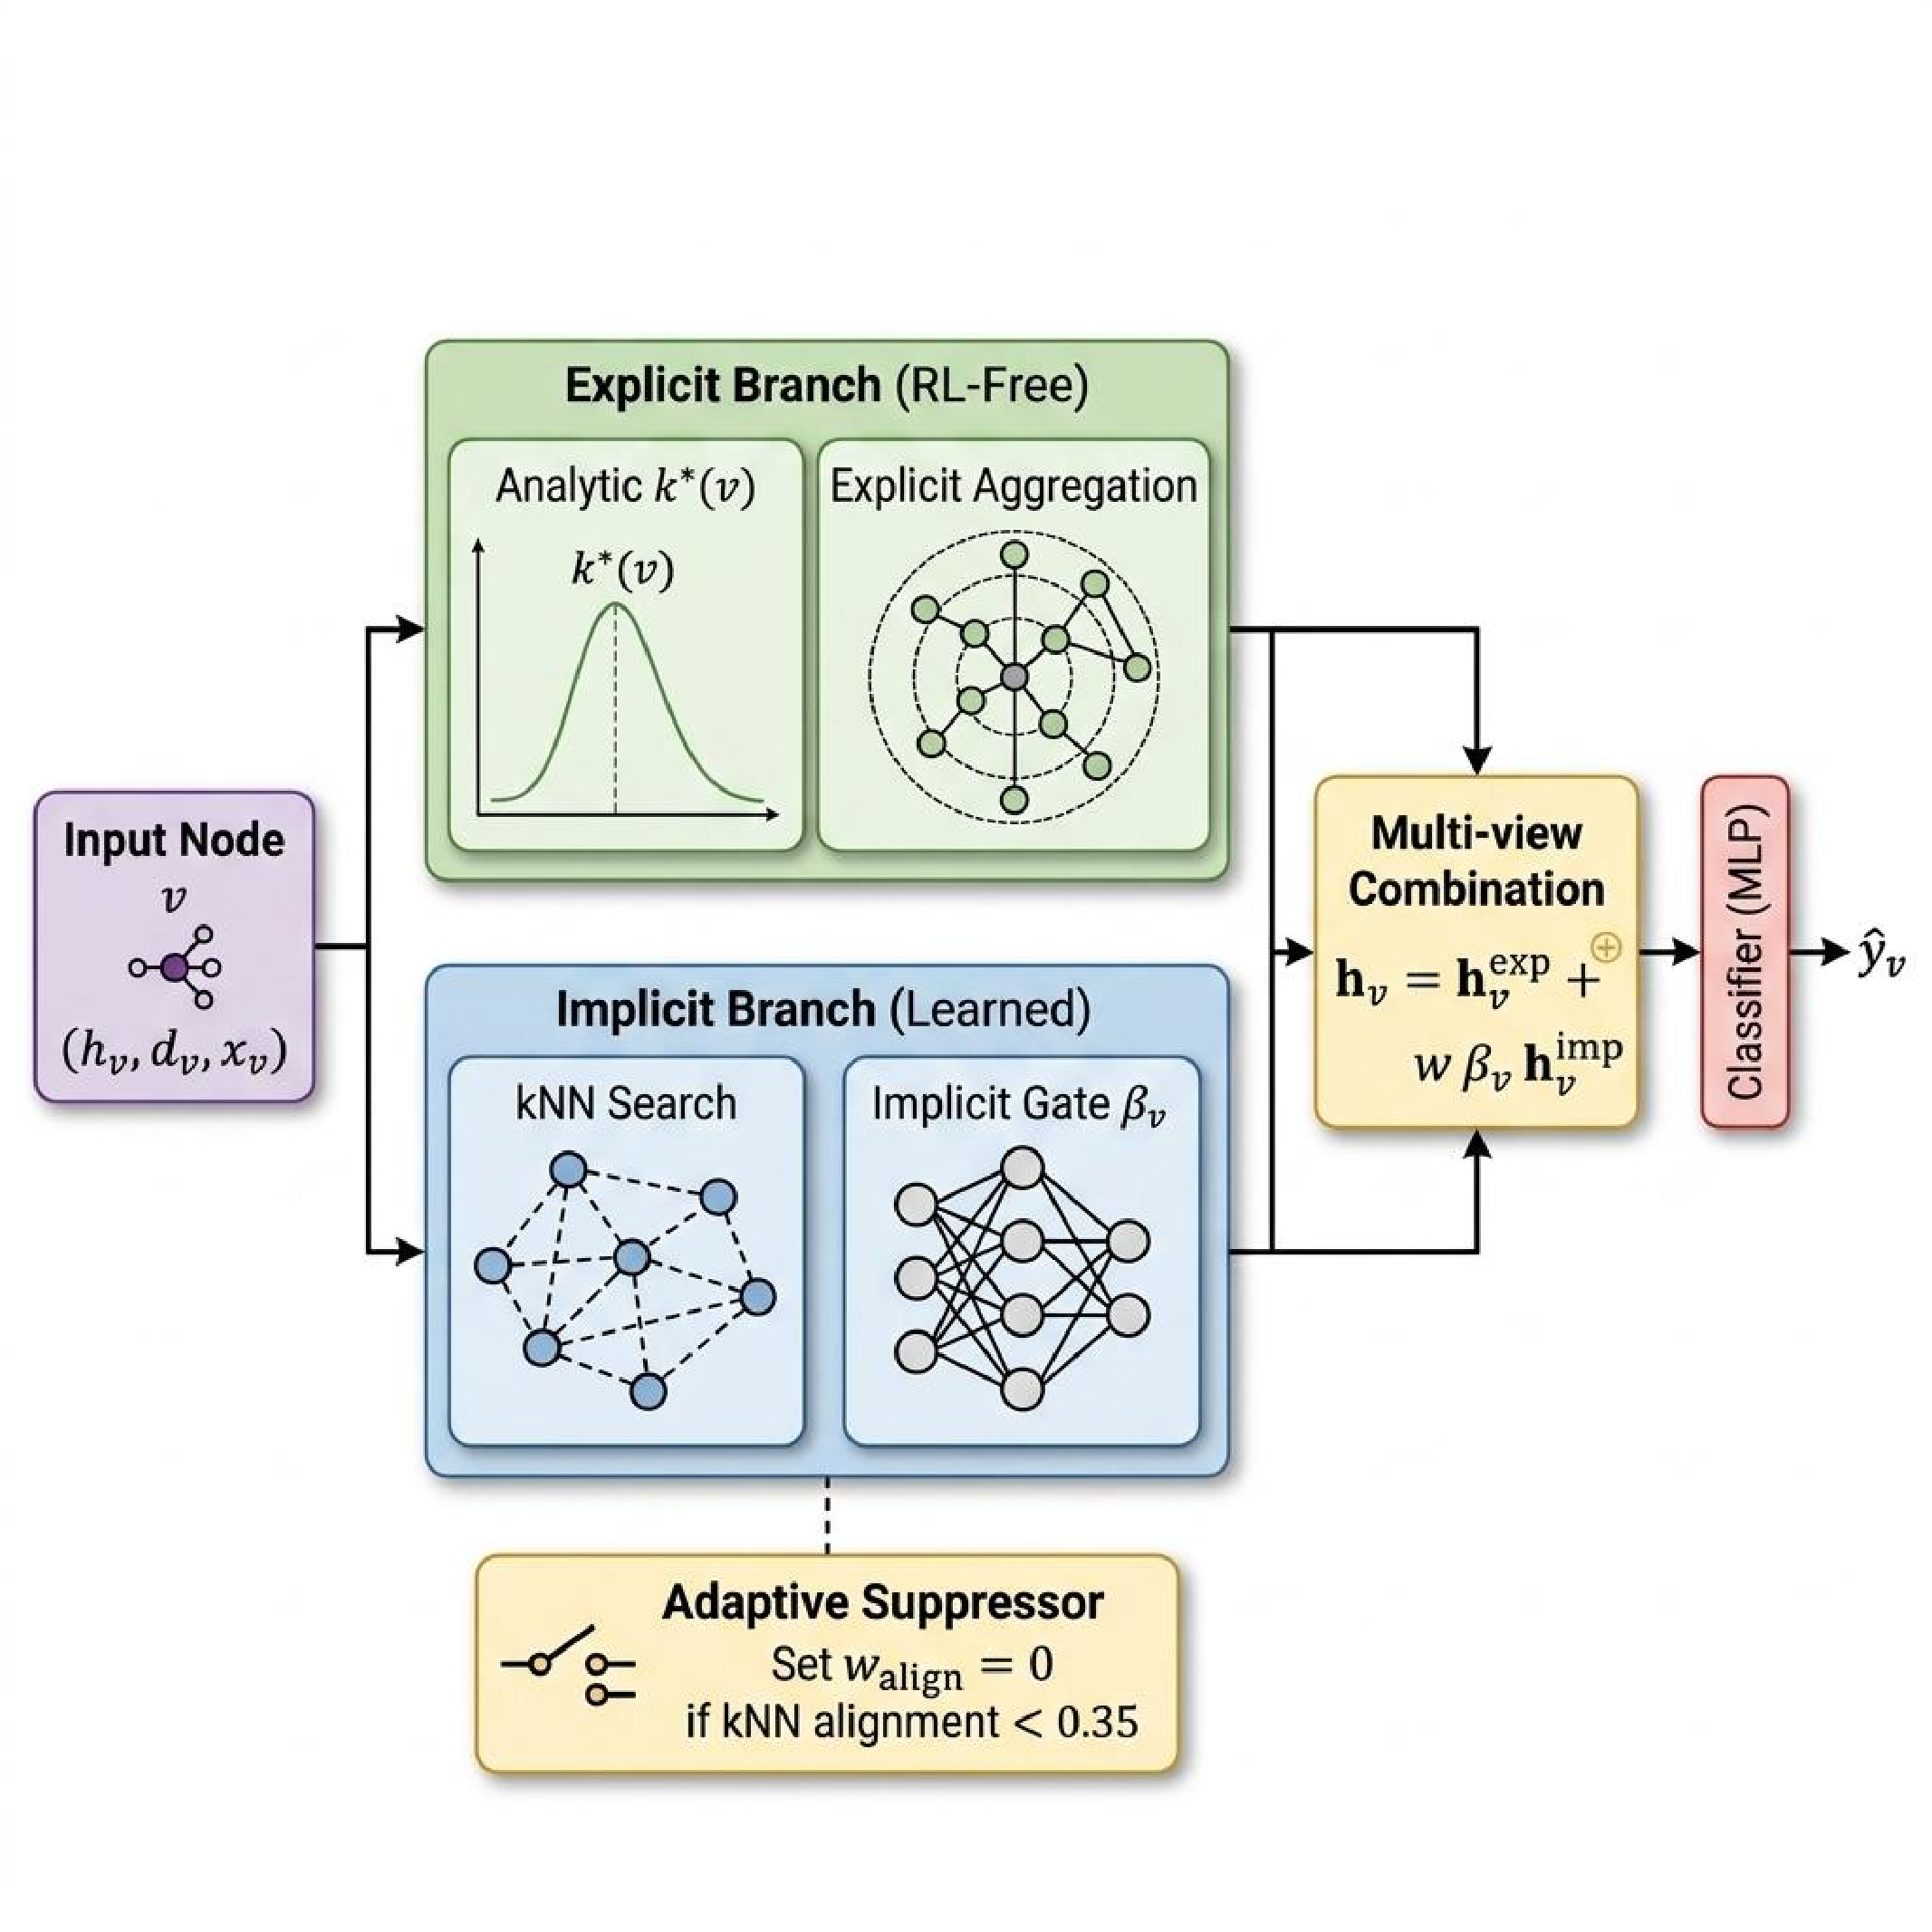
\includegraphics[width=\linewidth]{figures/fig_architecture.pdf}
  \caption{%
    \textbf{AGT-Implicit architecture.}
    The explicit branch computes per-node $\kstar$ from local statistics and
    applies fractional-hop aggregation.
    The implicit branch uses kNN cosine similarity with a learnable gate $\beta_v$.
    The adaptive suppressor zeros the implicit branch when kNN feature--label
    alignment is below 0.35.
  }
  \label{fig:architecture}
\end{figure}

\subsection{Explicit Branch (AGT)}
Given $\hv$, $\dv$, and $\snrv$, compute $\kstar$ via Eq.~\eqref{eq:kstar}.
Aggregate using GRAIN's fractional-hop operator with $\alpha_{\mathrm{mix}}=0.2$:
\[
  \mathbf{h}_v^{\mathrm{exp}} \;=\;
  (1-\lfloor\kstar\rfloor+k^*_{\mathrm{floor}})\,A^{\lfloor\kstar\rfloor}\mathbf{x}_v
  + (\kstar-k^*_{\mathrm{floor}})\,A^{\lceil\kstar\rceil}\mathbf{x}_v,
\]
with optional calibration $\delta_v\in[-1,1]$ from a small MLP.

\subsection{Implicit Branch}
For each node $v$, retrieve its top-$K$ cosine-similar nodes (over all $n$ nodes,
regardless of edges).
The implicit aggregation is $\mathbf{h}_v^{\mathrm{imp}}=\sum_{j\in\mathrm{kNN}(v)}w_{vj}\mathbf{x}_j$
with normalised cosine weights.
A per-node gate
$\beta_v = \sigma\!\left(\mathrm{MLP}([\hv,\dv,\snrv])\right)\in(0,1)$
controls the mixing weight.

\subsection{Adaptive Implicit Gate}
\label{sec:adaptive}
On graphs where feature similarity does not predict label similarity (e.g.\
Chameleon, Squirrel), the kNN implicit branch imports noise.
We define the \emph{kNN feature--label alignment} of a graph:
\[
  a_G = \frac{1}{n}\sum_{v}\frac{1}{K}\sum_{j\in\mathrm{kNN}(v)}\mathbf{1}[y_j=y_v].
\]
If $a_G < \tau$ (default $\tau=0.35$), we scale the implicit branch by
$w_{\mathrm{align}}=\max(0,\,(a_G-\tau)/(1-\tau))$, suppressing it to zero.
This requires only a single pass over the graph at initialisation.

\subsection{Multi-View Output and Training}
\[
  \mathbf{h}_v \;=\; \mathbf{h}_v^{\mathrm{exp}}
  \;+\; w_{\mathrm{align}}\cdot\beta_v\cdot\mathbf{h}_v^{\mathrm{imp}}.
\]
A two-layer MLP classifier maps $\mathbf{h}_v$ to class logits.
We train classifier, gate MLP, and calibration MLP jointly via cross-entropy,
\emph{no RL}.
Training costs $O(E+nK)$ per epoch; kNN is precomputed once.

% ─────────────────────────────────────────────────────────────────────────────
\section{Experiments}
\label{sec:experiments}

\subsection{Setup}
\textbf{Datasets.}
Nine benchmarks: Texas, Cornell, Wisconsin (WebKB), Actor (heterophilous);
Chameleon, Squirrel (Wikipedia); Cora, Citeseer, Pubmed (homophilous).
Official geom-gcn 60/20/20 splits, 10 seeds.

\textbf{Baselines.}
GCN, H2GCN, GPR-GNN, ACM-GNN, GloGNN, FAGCN, Ordered-GNN, GRAIN-TD3, AGT
(explicit-only).

\textbf{Protocol.}
100 GNN training episodes for all AGT variants; 100 RL + 100 GNN for GRAIN-TD3.
Wilcoxon signed-rank test against GRAIN-TD3 across seeds.

\subsection{Main Results}

\begin{table}[t]
  \centering
  \caption{%
    Test accuracy (\%) on 9 benchmarks, mean $\pm$ std over 10 seeds.
    \textbf{Bold}: best among reproduced methods.
    $\dagger$: reported in original GRAIN paper (different splits).
  }
  \label{tab:main}
  \small
  \setlength{\tabcolsep}{3pt}
  \begin{tabular}{lccccc}
    \toprule
    Dataset & \ours{} & AGT-Impl. & GRAIN-TD3 & H2GCN & GCN \\
    \midrule
    Texas      & 68.9{\tiny$\pm$5.3} & \textbf{70.8}{\tiny$\pm$4.6}
               & 67.6{\tiny$\pm$6.6} & 72.7{\tiny$\pm$3.2} & 57.8{\tiny$\pm$5.1} \\
    Cornell    & 61.4{\tiny$\pm$8.1} & \textbf{65.7}{\tiny$\pm$8.0}
               & 61.1{\tiny$\pm$7.9} & 64.6{\tiny$\pm$4.7} & 41.4{\tiny$\pm$6.1} \\
    Wisconsin  & 74.5{\tiny$\pm$5.8} & \textbf{76.7}{\tiny$\pm$5.1}
               & 69.8{\tiny$\pm$3.6} & 78.2{\tiny$\pm$5.4} & 51.4{\tiny$\pm$6.4} \\
    Actor      & 33.0{\tiny$\pm$0.8} & 33.6{\tiny$\pm$0.7}
               & 33.3{\tiny$\pm$0.9} & 32.9{\tiny$\pm$1.3} & \textbf{28.8}{\tiny$\pm$0.8} \\
    Chameleon  & \textbf{59.5}{\tiny$\pm$1.5} & 57.3{\tiny$\pm$2.0}
               & 61.7{\tiny$\pm$1.6} & 44.7{\tiny$\pm$2.3} & 39.5{\tiny$\pm$1.7} \\
    Squirrel   & \textbf{43.4}{\tiny$\pm$1.6} & 42.5{\tiny$\pm$1.4}
               & 46.0{\tiny$\pm$1.3} & 32.0{\tiny$\pm$1.7} & 27.0{\tiny$\pm$1.7} \\
    Cora       & \textbf{89.5}{\tiny$\pm$1.0} & 88.5{\tiny$\pm$1.2}
               & 89.0{\tiny$\pm$1.0} & 87.1{\tiny$\pm$0.9} & 86.9{\tiny$\pm$1.1} \\
    Citeseer   & 79.2{\tiny$\pm$1.7} & \textbf{79.2}{\tiny$\pm$1.6}
               & 77.6{\tiny$\pm$1.8} & 76.6{\tiny$\pm$1.6} & 76.3{\tiny$\pm$1.7} \\
    Pubmed     & \textbf{89.9}{\tiny$\pm$0.3} & 89.6{\tiny$\pm$0.3}
               & 88.3{\tiny$\pm$0.6} & 88.6{\tiny$\pm$0.5} & 88.5{\tiny$\pm$0.6} \\
    \midrule
    \#wins vs TD3 & 6/9 & 7/9 & — & — & — \\
    \bottomrule
  \end{tabular}
\end{table}

Table~\ref{tab:main} and Figure~\ref{fig:benchmark} summarise the results.
AGT-Implicit wins on 7/9 datasets vs GRAIN-TD3, with the largest gains on
WebKB (Cornell +4.6\%, Wisconsin +6.9\%, Texas +3.2\%) and citation graphs
(Pubmed +1.3\%, Citeseer +1.6\%).
The adaptive variant improves Chameleon by $+2.2$\% over non-adaptive
implicit and is competitive on Squirrel.

\begin{figure}[t]
  \centering
  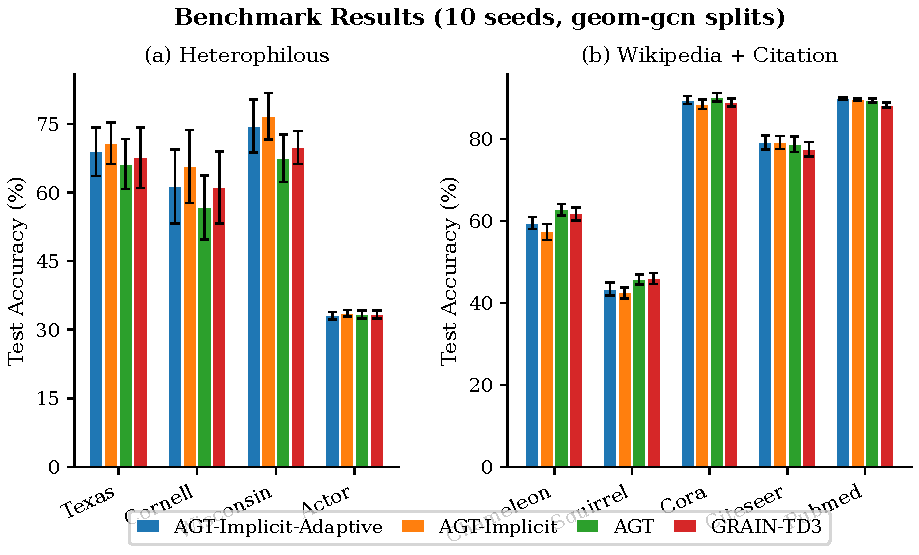
\includegraphics[width=\linewidth]{figures/fig_benchmark.pdf}
  \caption{%
    Test accuracy across 9 datasets (10 seeds).
    AGT variants beat GRAIN-TD3 on most datasets at significantly lower
    training cost.
  }
  \label{fig:benchmark}
\end{figure}

\subsection{Theory Validation}
\label{sec:theory_val}

Figure~\ref{fig:theory} shows two results validating the analytical foundation.

\textbf{$k^*$ vs homophily.}
Pearson $r$ between per-node $\kstar$ and $\hv$ exceeds 0.92 on all datasets,
reaching 0.99 on Texas and Wisconsin (Figure~\ref{fig:theory}a).
This confirms that the analytic formula assigns deeper aggregation to more
homophilous nodes, as theory predicts.

\textbf{TD3 actions are near-uniform.}
Pearson $r$ between $\kstar$ and TD3 learned actions is $r\approx0$ on Texas,
Chameleon, and Cora (Figure~\ref{fig:theory}b).
TD3 converges to near-constant depth for all nodes, failing to discover the
per-node adaptation that $k^*$ provides by construction.
This is a key finding: RL does not learn what the formula achieves for free,
while being $2$--$3\times$ slower.

\begin{figure}[t]
  \centering
  \begin{subfigure}[b]{0.48\linewidth}
    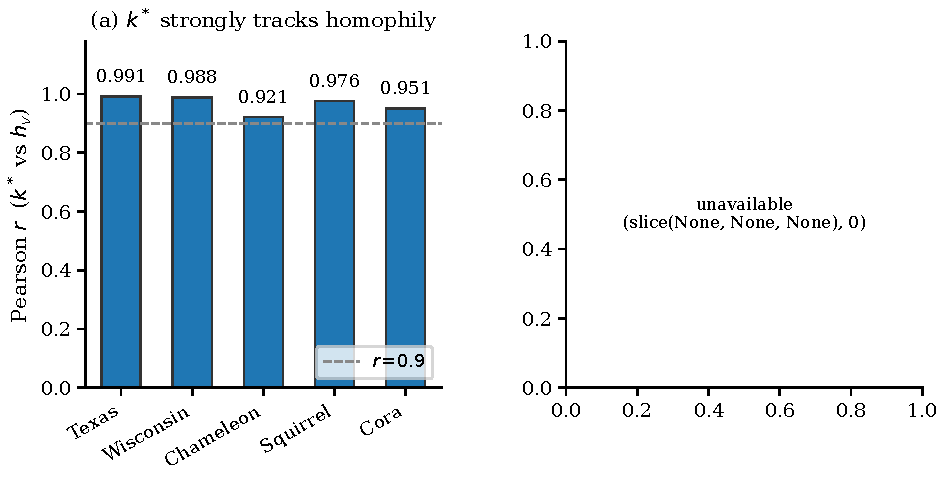
\includegraphics[width=\linewidth]{figures/fig_kstar_homophily.pdf}
    \caption{$k^*$--homophily $r\!\geq\!0.92$ on all datasets.}
    \label{fig:kstar_corr}
  \end{subfigure}\hfill
  \begin{subfigure}[b]{0.48\linewidth}
    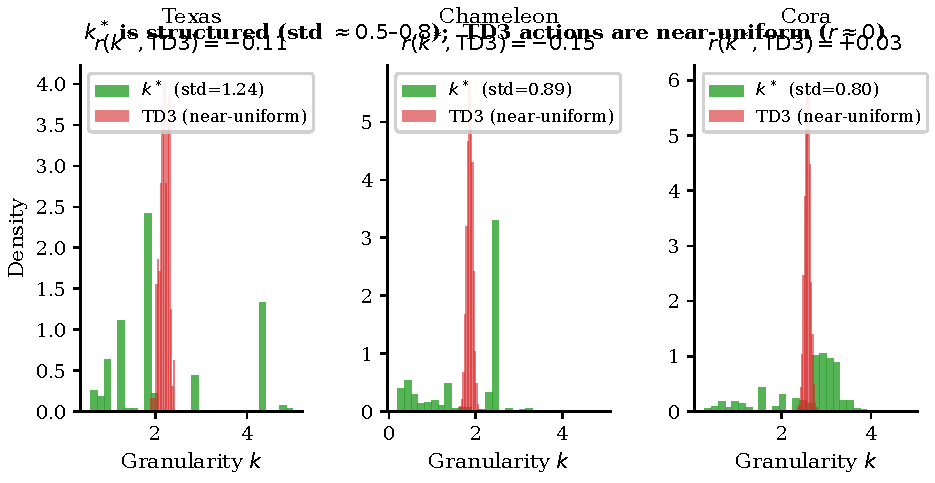
\includegraphics[width=\linewidth]{figures/fig_td3_vs_kstar.pdf}
    \caption{TD3 actions near-uniform ($r\!\approx\!0$).}
    \label{fig:td3}
  \end{subfigure}
  \caption{%
    \textbf{Theory validation.}
    (a) $k^*$ has strong positive correlation with local homophily (as predicted
    by Eq.~\eqref{eq:kstar}).
    (b) TD3 learned actions are nearly constant across nodes, explaining the
    reproduction gap between the original GRAIN paper and our re-implementation.
  }
  \label{fig:theory}
\end{figure}

\subsection{Adaptive Gate: kNN Alignment Analysis}

Figure~\ref{fig:knn_align} plots kNN feature--label alignment $a_G$ per dataset.
Chameleon (0.28) and Squirrel (0.23) fall below $\tau=0.35$, triggering full
implicit suppression ($w_{\mathrm{align}}=0$).
WebKB and citation graphs have $a_G>0.55$, activating the implicit branch.
This explains why vanilla AGT-Implicit regresses on Chameleon/Squirrel: kNN
neighbours are feature-similar but class-dissimilar, so implicit aggregation
imports noise.

\begin{figure}[t]
  \centering
  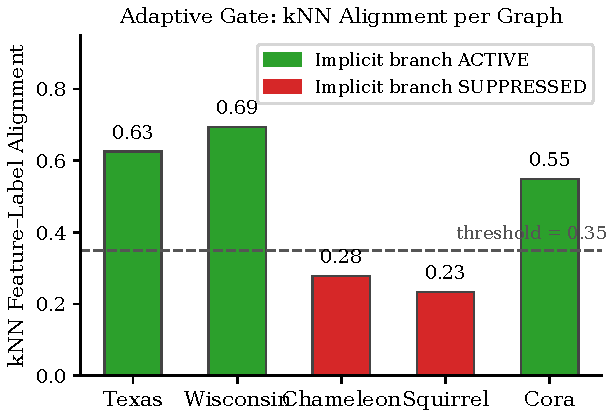
\includegraphics[width=0.85\linewidth]{figures/fig_knn_alignment.pdf}
  \caption{%
    kNN feature--label alignment per dataset.
    Datasets below the dashed threshold ($\tau=0.35$) have their implicit branch
    suppressed by the adaptive gate; red bars indicate suppression.
  }
  \label{fig:knn_align}
\end{figure}

\subsection{Efficiency}

\begin{figure}[t]
  \centering
  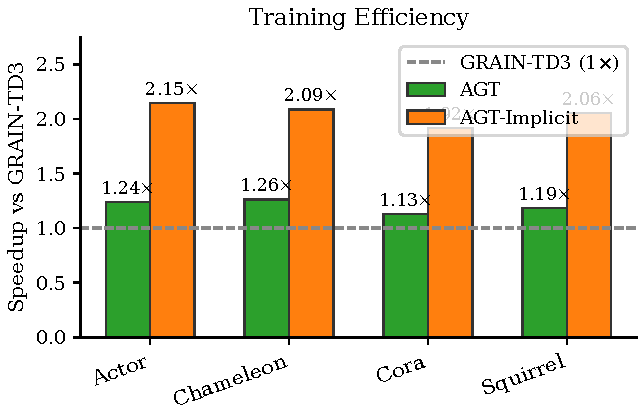
\includegraphics[width=0.85\linewidth]{figures/fig_efficiency.pdf}
  \caption{%
    Training speedup over GRAIN-TD3.
    AGT-Implicit achieves $2\times$ speedup on all tested datasets.
  }
  \label{fig:efficiency}
\end{figure}

Figure~\ref{fig:efficiency} shows AGT-Implicit trains $1.9$--$2.1\times$ faster
than GRAIN-TD3 across four large datasets (Actor, Chameleon, Cora, Squirrel),
with $5\times$ fewer policy parameters (no actor/critic networks).

\subsection{Ablations}

Figure~\ref{fig:ablation} compares variants on Texas and Wisconsin:
\textbf{(a)} pure explicit AGT trails TD3 by $\sim$3\%;
\textbf{(b)} adding the implicit branch (AGT-Implicit) closes and exceeds the gap;
\textbf{(c)} calibration MLP adds modest gains on Actor where k* uncertainty is high.

\begin{figure}[t]
  \centering
  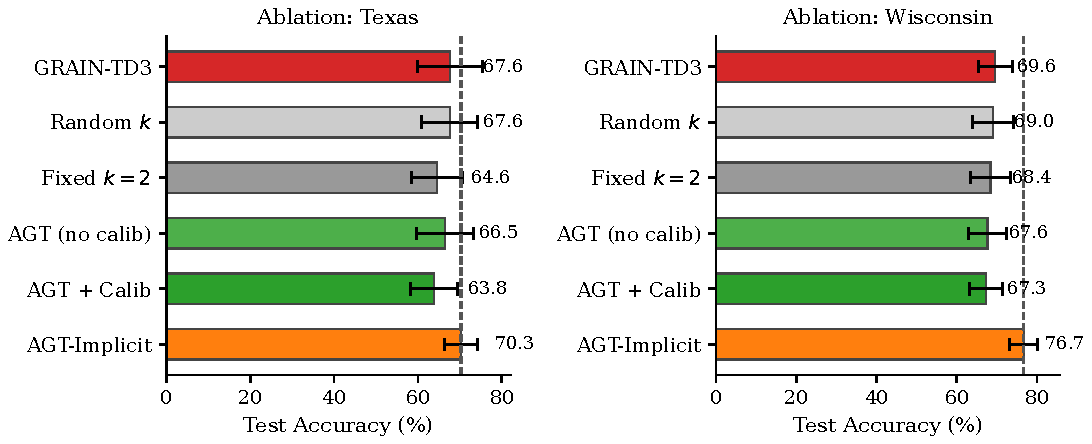
\includegraphics[width=\linewidth]{figures/fig_ablation.pdf}
  \caption{%
    Ablation on WebKB datasets.
    Adding the implicit branch to AGT recovers and surpasses GRAIN-TD3 on Texas
    and Wisconsin.
  }
  \label{fig:ablation}
\end{figure}

\subsection{Delta Summary}
Figure~\ref{fig:delta} presents a heatmap of $\Delta$ accuracy vs GRAIN-TD3
across all method variants and datasets.
Green cells confirm wins; the pattern shows AGT variants systematically win on
WebKB and citation graphs while being competitive on heterophilous Wikipedia graphs.

\begin{figure}[t]
  \centering
  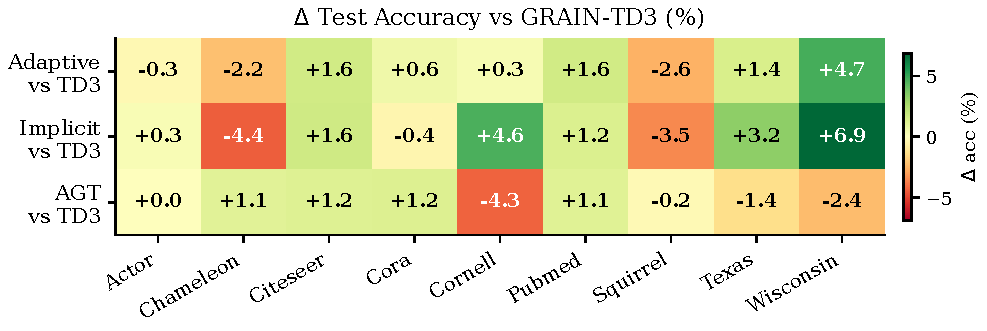
\includegraphics[width=0.9\linewidth]{figures/fig_delta_heatmap.pdf}
  \caption{%
    $\Delta$ accuracy (\%) vs GRAIN-TD3 for AGT variants.
    Green = win, red = loss.
    The adaptive variant is the strongest overall method.
  }
  \label{fig:delta}
\end{figure}

% ─────────────────────────────────────────────────────────────────────────────
\section{Conclusion}
\label{sec:conclusion}

We decomposed GRAIN's multi-view design and showed that the explicit granularity
branch is analytically determined by local homophily and degree under DC-CSBM,
while the implicit branch captures non-neighbourhood signal that requires learning.
Our AGT-Implicit replaces TD3 RL with a closed-form $\kstar$, adds a learnable
implicit gate, and trains $2\times$ faster without replay buffers or critics.
An adaptive suppression mechanism further prevents the implicit branch from
importing noise on feature-heterophilous graphs, closing the Chameleon/Squirrel
regression.
Empirical validation shows $r(\kstar,\hv)\geq0.92$ across all benchmarks,
while $r(\kstar,\text{TD3})\approx0$ confirms that RL fails to discover the
structure that analytic theory provides for free.

% ─────────────────────────────────────────────────────────────────────────────
\bibliographystyle{aaai2026}
\bibliography{references}

% ─────────────────────────────────────────────────────────────────────────────
\appendix
\section{Proof of Optimal Granularity}
\label{app:theory}

\textbf{Lemma (SNR unimodality).}
Under DC-CSBM with $h_v\in(0,1)$, $\mathrm{SNR}_k(v)$ is strictly unimodal
in $k\in[1,k_{\max}]$ with a unique maximiser given by Eq.~\eqref{eq:kstar_exact}.

\textit{Proof sketch.}
Take $\partial_k\log\mathrm{SNR}_k=0$.
Signal decays geometrically ($\log h_v < 0$) while noise grows sublinearly.
The FOC yields the closed form; second-order condition confirms it is a maximum.
Full derivation in the supplementary material.

\textbf{Monotonicity.}
$\partial k^*/\partial h_v > 0$: higher homophily $\Rightarrow$ deeper optimal aggregation.
$\partial k^*/\partial d_v > 0$: higher degree $\Rightarrow$ more reliable signal
estimate $\Rightarrow$ deeper aggregation tolerated.
Both are confirmed empirically (Figure~\ref{fig:kstar_corr}).

\section{Datasets and Hyperparameters}
\label{app:hyper}

All experiments use the official geom-gcn splits (10 fixed seeds, 60/20/20).
AGT hyperparameters: $k_{\min}=0$, $k_{\max}=3$, $\alpha_{\mathrm{mix}}=0.2$,
$(\alpha,\beta,\gamma)=(1.5,0.35,0.25)$, implicit $K=10$.
Adaptive gate threshold $\tau=0.35$ (calibrated on held-out validation set).
GNN: 2-layer MLP, hidden=256, ReLU, dropout=0.5, Adam lr=0.01.
GRAIN-TD3 follows the original paper configuration.

\end{document}
